This chapter describes the implementation of the GitHub issue classification system, including the common data pipeline, model families, evaluation components, and experiment-execution process. The main goal of the implementation is to keep data handling and evaluation consistent while allowing each model family to use its own training procedure.

\section{Project Architecture}
The system is organized into components responsible for data loading, preprocessing, model training, inference, evaluation, and result storage. The dataset service reads GitHub issue records and converts them into a common representation containing the repository, issue title, issue body, and target label. The title and body are then combined into the textual input used by the selected model.

\begin{figure}[h]
\centering
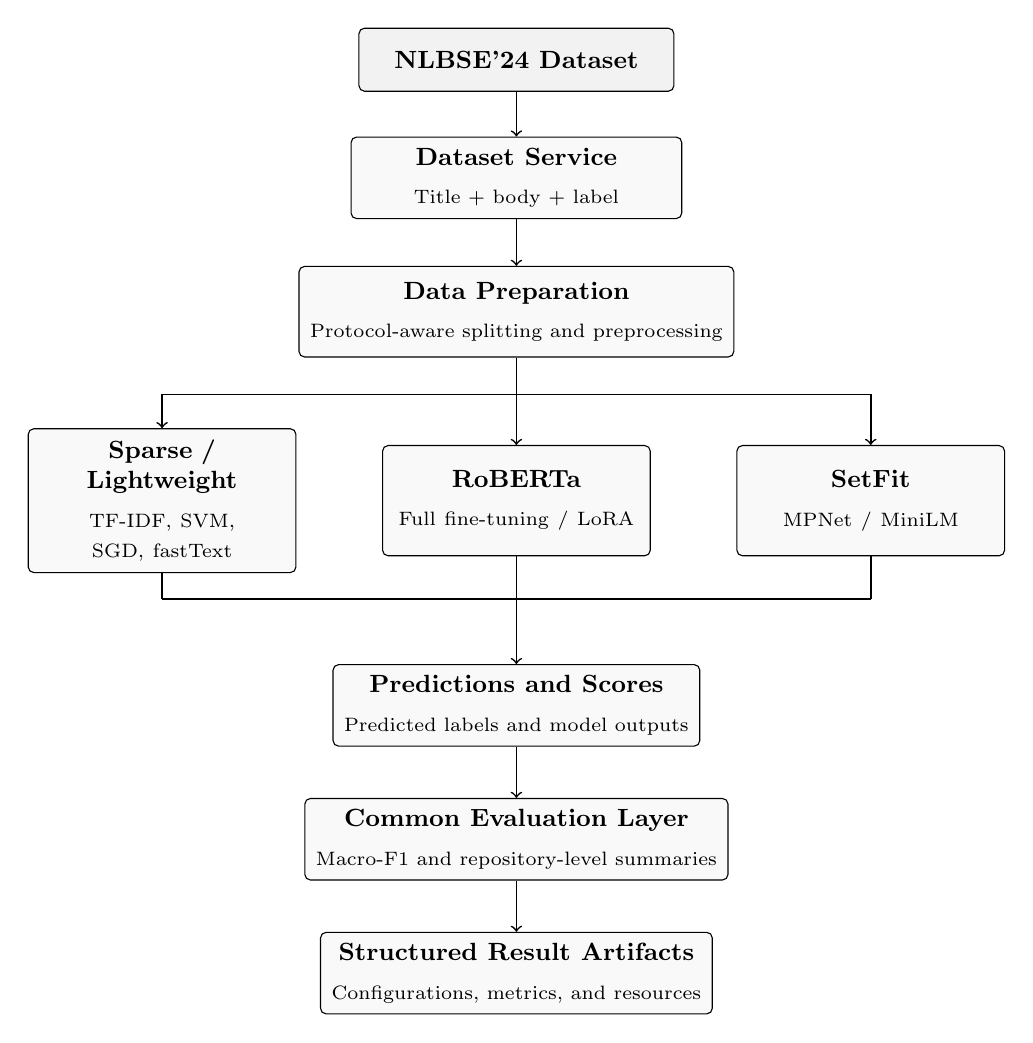
\begin{tikzpicture}[
    box/.style={
        draw,
        rounded corners=2pt,
        align=center,
        fill=gray!5,
        inner sep=4pt,
        font=\small
    },
    arrow/.style={
        ->,
        semithick
    }
]

% ==================================================
% Top pipeline
% ==================================================

\node[
    box,
    fill=gray!10,
    minimum width=4.0cm,
    minimum height=0.8cm
] (data) at (0,7.0)
{\textbf{NLBSE'24 Dataset}};


\node[
    box,
    minimum width=4.2cm,
    minimum height=1.0cm
] (service) at (0,5.5)
{
    \textbf{Dataset Service}\\[1mm]
    {\scriptsize Title + body + label}
};


\node[
    box,
    minimum width=4.2cm,
    minimum height=1.15cm
] (prep) at (0,3.8)
{
    \textbf{Data Preparation}\\[1mm]
    {\scriptsize Protocol-aware splitting and preprocessing}
};


% ==================================================
% Model boxes
% ==================================================

\node[
    box,
    text width=3.0cm,
    minimum width=3.4cm,
    minimum height=1.4cm
] (sparse) at (-4.5,1.4)
{
    \textbf{Sparse / Lightweight}\\[1mm]
    {\scriptsize TF-IDF, SVM, SGD, fastText}
};


\node[
    box,
    text width=3.0cm,
    minimum width=3.4cm,
    minimum height=1.4cm
] (roberta) at (0,1.4)
{
    \textbf{RoBERTa}\\[1mm]
    {\scriptsize Full fine-tuning / LoRA}
};


\node[
    box,
    text width=3.0cm,
    minimum width=3.4cm,
    minimum height=1.4cm
] (setfit) at (4.5,1.4)
{
    \textbf{SetFit}\\[1mm]
    {\scriptsize MPNet / MiniLM}
};


% ==================================================
% Results pipeline
% ==================================================

\node[
    box,
    minimum width=4.3cm,
    minimum height=1.0cm
] (pred) at (0,-1.2)
{
    \textbf{Predictions and Scores}\\[1mm]
    {\scriptsize Predicted labels and model outputs}
};


\node[
    box,
    minimum width=4.3cm,
    minimum height=1.0cm
] (eval) at (0,-2.9)
{
    \textbf{Common Evaluation Layer}\\[1mm]
    {\scriptsize Macro-F1 and repository-level summaries}
};


\node[
    box,
    minimum width=4.3cm,
    minimum height=1.0cm
] (artifact) at (0,-4.6)
{
    \textbf{Structured Result Artifacts}\\[1mm]
    {\scriptsize Configurations, metrics, and resources}
};


% ==================================================
% Top arrows
% ==================================================

\draw[arrow] (data.south) -- (service.north);
\draw[arrow] (service.south) -- (prep.north);


% ==================================================
% Split into three model families
% ==================================================

% Vertical stem
\draw[semithick] (prep.south) -- (0,2.75);

% Horizontal branch
\draw[semithick] (-4.5,2.75) -- (4.5,2.75);

% Arrows down to models
\draw[arrow] (-4.5,2.75) -- (sparse.north);
\draw[arrow] (0,2.75) -- (roberta.north);
\draw[arrow] (4.5,2.75) -- (setfit.north);


% ==================================================
% Merge model outputs
% ==================================================

% Vertical outputs from models
\draw[semithick] (sparse.south) -- (-4.5,0.15);
\draw[semithick] (roberta.south) -- (0,0.15);
\draw[semithick] (setfit.south) -- (4.5,0.15);

% Horizontal merge line
\draw[semithick] (-4.5,0.15) -- (4.5,0.15);

% Arrow to predictions
\draw[arrow] (0,0.15) -- (pred.north);


% ==================================================
% Final pipeline
% ==================================================

\draw[arrow] (pred.south) -- (eval.north);
\draw[arrow] (eval.south) -- (artifact.north);

\end{tikzpicture}

\caption{High-level architecture of the experimental pipeline.}
\label{fig:project-architecture}
\end{figure}

The experiment pipeline separates data preparation from model-specific training. After the dataset is loaded, the selected evaluation protocol determines how training and validation examples are divided. Components that learn from the data, such as TF-IDF vectorizers, are fitted only on the training partition of each experiment. Figure~\ref{fig:project-architecture} shows how the different model families share the same data and evaluation layers.

A common evaluation component is applied after inference. Predictions are associated with their original issue identifiers, repositories, folds, and target labels before metrics are calculated. Experimental outputs are stored as structured artifacts containing model configurations, predictions, scores, resource measurements, and environment information. This organization reduces manual copying of results and makes later comparison easier.

\section{Persistence and Team Contributions}
The \texttt{IssueRepository} abstraction is shared by in-memory, CSV and JSON adapters. \texttt{IssueDatasetService} and the runner consume this interface, so changing persistence does not require changing model/evaluation logic. This implements interchangeable memory/file storage.

\begin{table}[H]
\centering\small
\caption{Implementation ownership; each member also owns their module's analysis.}
\begin{tabularx}{\textwidth}{l l X}
\toprule
Owner & Member & Contribution \\
\midrule
P1 & Pham Tuan Kiet & Leadership; data/persistence, splits, contracts, Logistic Regression and text ablations. \\
P2 & Nguyen Trung Hieu & Sparse models, fastText, tuning and feature ablations. \\
P3 & Le Ngoc Anh & RoBERTa full/LoRA, per-repository and pooled experiments. \\
P4 & Nguyen Hoang Nam & SetFit MPNet/MiniLM, few-shot and iteration ablations. \\
P5 & Bui Tien Dung & Aggregation, paired comparisons, ensemble/resource utilities, demo and report integration. \\
\bottomrule
\end{tabularx}
\end{table}

\section{TF-IDF Logistic Regression Baseline}
The baseline classifier uses TF-IDF to transform issue text into a sparse numerical representation. The title and body are concatenated before feature extraction. Word-level unigrams and bigrams are used so that the representation can capture both individual technical terms and short phrases that may indicate issue intent. The TF-IDF vectorizer is fitted exclusively on the training portion of each fold and is then applied to the corresponding validation data.

Logistic Regression is trained on the resulting sparse feature vectors to predict the three target classes: bug, feature, and question. This model provides a computationally inexpensive reference for evaluating whether more complex contextual models produce useful gains.

A title-only configuration is also evaluated as an ablation. The model and feature extraction procedure remain unchanged while the issue body is removed from the input. The comparison measures how much useful information is contributed by the detailed issue description.

\section{Lightweight Text Classification Models}
Several lightweight classifiers are implemented as alternatives to the Logistic Regression baseline. LinearSVC is evaluated with both word-only TF-IDF features and a combination of word and character features. Character n-grams can preserve information from source-code identifiers, file paths, error messages, package names, and version strings that may be fragmented by conventional tokenization.

Complement Naive Bayes and a hashing-based Stochastic Gradient Descent classifier provide additional sparse-learning alternatives. The hashing-based model maps textual features into a fixed-dimensional space without maintaining an explicit vocabulary. A supervised fastText model is also included as a lightweight neural approach that can use subword information.

\section{RoBERTa Full Fine-Tuning}
RoBERTa-base is used as the main pretrained Transformer classifier. Each issue is formed by concatenating its title and body before tokenization. The tokenizer converts the text into subword token identifiers and an attention mask. Input sequences are truncated to a maximum length of 160 tokens to maintain a consistent computational budget across the reported RoBERTa experiments.

For full fine-tuning, the pretrained encoder is combined with a three-class classification head. Gradients are propagated through both the classification head and the pretrained Transformer layers. RoBERTa is evaluated under repository-specific and pooled cross-validation so that repository-specific training and multi-repository training can be examined separately.

\section{RoBERTa with LoRA}
The parameter-efficient RoBERTa configuration uses LoRA adapters in selected attention projections. Most pretrained RoBERTa weights remain frozen, while the low-rank adapter parameters and task-specific classification components are optimized. The tokenizer, maximum sequence length, and three-class prediction objective are kept aligned with the full fine-tuning configuration to make the adaptation strategies easier to compare.

The LoRA configuration is evaluated in the same repository-aware framework as full RoBERTa. Repository-level results are preserved before aggregate scores are calculated.

\section{SetFit Classification}
SetFit is implemented using Sentence Transformer encoders. In the first stage, the sentence encoder is adapted through contrastive training. In the second stage, the adapted encoder generates dense embeddings and a lightweight classification head is fitted on these representations.

Two encoder backbones are considered: MPNet and MiniLM. Additional experiments vary the number of labeled training examples with $k=8$, $k=16$, and $k=32$, and vary the number of contrastive-training iterations. These configurations are used to study the relationship between data availability, additional training effort, and predictive performance.

\section{Configuration Summary}
Few-shot $k$ denotes examples \emph{per class}: 24, 48 or 96 examples per repository/fold for $k=8,16,32$. ``Full data'' uses only each CV fold's training partition (approximately 240 issues), not all 300 issues including validation.

Table~\ref{tab:configuration-summary} collects the model settings that are explicitly discussed in this report. More detailed run-specific information is stored in the experiment artifacts generated by the implementation.

\begin{table}[H]
\centering
\caption{Summary of the main reported model configurations.}
\label{tab:configuration-summary}
\begin{tabularx}{\textwidth}{>{\bfseries}l X}
\toprule
Model family & Reported configuration \\
\midrule
TF-IDF + Logistic Regression & Word unigrams and bigrams; title + body; title-only ablation \\
LinearSVC & Word-only and word + character feature variants \\
Hashed SGD & Hashing-based sparse text representation \\
fastText & Supervised word/subword text classifier \\
RoBERTa & RoBERTa-base; maximum sequence length of 160 tokens; full fine-tuning \\
RoBERTa + LoRA & Same input setup as full RoBERTa; parameter-efficient low-rank adapters \\
SetFit & MPNet and MiniLM backbones; $k \in \{8,16,32\}$ experiments; multiple contrastive-iteration settings \\
\bottomrule
\end{tabularx}
\end{table}

P1/P3/P4 runs reported here use seed 42. Logistic Regression uses word 1--2 grams, minimum document frequency 2, at most 50,000 features, $C=4$, balanced weights and LBFGS (maximum 2,000 iterations). RoBERTa uses 20 epochs, train/evaluation batches 16/32 and maximum length 160. Full fine-tuning uses learning rate $2\times10^{-5}$ and weight decay 0.1; LoRA uses $3\times10^{-4}$ and weight decay 0, rank 48, alpha 96, dropout 0.1, targeting query/key/value and attention-output dense projections. These are different recipes, so differences cannot be attributed solely to the adapter mechanism. SetFit uses maximum length 128, one epoch, encoder/head batches 16/2, and 20 iterations unless ablated. Exact configurations are versioned under \texttt{configs/}.

\section{Evaluation, Ensemble, and Resource Utilities}
All trained models are evaluated through a common component. Macro-F1 is the primary performance metric, while repository-level results are retained before aggregate summaries are computed. This avoids hiding large differences between repositories behind a single overall value.

The implementation also supports paired bootstrap analysis when two models provide predictions for the same examples. Resampling matched predictions can be used to estimate uncertainty in the observed difference between models. In addition, ensemble utilities support hard voting on predicted labels and soft voting when compatible probability outputs are available. Decision margins from models such as LinearSVC are not treated as probabilities without calibration.

Training time, inference time, and memory consumption are recorded when available. Resource measurements are interpreted cautiously because CPU/GPU hardware and the number of model-fitting operations differ across protocols. For this reason, values collected under different environments are treated as practical measurements rather than as a fully controlled benchmark.

\section{Experiment Execution}
Each experiment follows the same general sequence. The required split is created according to the selected evaluation protocol. Model-specific preprocessing is then fitted using only the training partition. The classifier is trained, predictions are generated for the validation or test partition, and the outputs are passed to the shared evaluation component. Metrics, predictions, resource measurements, and configuration information are stored together.

Repeating this process across repositories, folds, model configurations, and protocols produces the collection of artifacts used in the final analysis. The standardized procedure reduces the risk that observed differences arise from inconsistent data handling and makes the experimental workflow easier to verify and reproduce.
